\section{Resultados Experimentais}
    \begin{frame}[fragile]{Disposição do Dataset}
        \begin{figure}[H]
            \begin{center}
            \begin{tikzpicture}
                \begin{axis}[
                        ybar,
                        width=10.5cm,
                        height=6.5cm,
                        grid=both, 
                        bar width=8pt,
                        axis lines*=left,
                        ylabel=Quantidade,
                        % xlabel=Classes,
                        symbolic x coords={0,50,100,150,200},
                        ytick={0, 50, 100, 150, 200, 250, 300, 350},
                        % legend columns=2, 
                        % legend style={at={(0.6,1.0)},anchor=north west},
                        % legend style={at={(0,1.1)},anchor=north west},
                        xtick=data,
                    ]
                    % \addlegendentry{Comp. I}
                    \addplot[draw=black, pattern color=blue, pattern=horizontal lines] coordinates{
                        (0,91)
                        (50,105)
                        (100,162)
                        (150,77)
                        (200,255)
                    };

                    % \addlegendentry{Comp. II}
                    \addplot[draw=black, pattern color=green, pattern=vertical lines] coordinates{
                        (0,92)
                        (50,137)
                        (100,249)
                        (150,163)
                        (200,49)
                    };

                    % \addlegendentry{Comp. III}
                    \addplot[draw=black, pattern color=red, pattern=north east lines, preaction={draw=red, line width=2pt}] coordinates{
                        (0,138)
                        (50,138)
                        (100,138)
                        (150,138)
                        (200,138)
                    };

                    % \addlegendentry{Comp. IV}
                    \addplot[draw=black, pattern color=yellow, pattern=dots] coordinates{
                        (0,91)
                        (50,142)
                        (100,307)
                        (150,118)
                        (200,32)
                    };

                    % \addlegendentry{Comp. V}
                    \addplot[draw=black, pattern color=gray, pattern=grid] coordinates{
                        (0,97)
                        (50,170)
                        (100,149)
                        (150,155)
                        (200,119)
                    };
                    \legend{,,Competência III,,,};

                \end{axis}
            \end{tikzpicture}
            \captionsetup{labelformat=empty}
            \caption{Distribuição das classes sobre a \textbf{competência III} de \textbf{690 
            redações} no \textit{dataset} balanceado. Cada classe da competência 
            III possui uma amostragem de \textbf{138 textos}.}
            \label{graphic:dataset_balanced}
            \end{center}
        \end{figure}
    \end{frame}

    \begin{frame}[fragile]{Área Sobre a Curva ROC}
    \begin{figure}[H]
        \begin{center}
            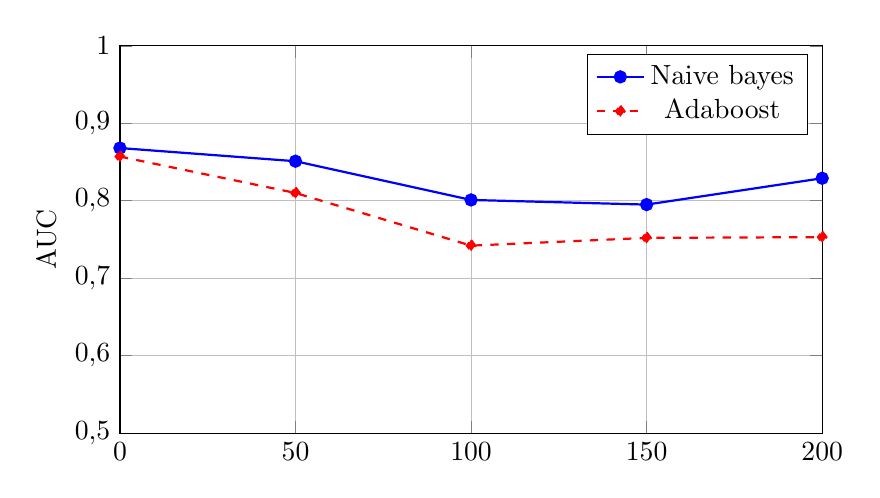
\begin{tikzpicture}
            \begin{axis}[width=10.5cm, 
                    height=6.5cm, 
                    grid=both, 
                    ymin=0.500, ymax=1.000,
                    xmin=0, xmax=200,
                    ylabel={AUC},
                    symbolic x coords={0,50,100,150,200},
                    ytick={0.500, 0.600, 0.700, 0.800, 0.900, 1.000},
                    xtick=data
                ]

                \addlegendentry{Naive bayes}
                \addplot[mark=*,thick,blue, solid] coordinates {
                (0,0.868) 
                (50,0.851) 
                (100,0.801) 
                (150,0.795) 
                (200,0.829) 
                };

                \addlegendentry{Adaboost}
                \addplot[mark=diamond*,thick,red, dashed] coordinates {
                (0,0.857) 
                (50,0.810) 
                (100,0.742) 
                (150,0.752) 
                (200,0.753) 
                };

            \end{axis}
            \end{tikzpicture}
        \end{center}
        \captionsetup{labelformat=empty}
        \caption{O pontos da área sob curva ROC demonstra o \textbf{poder 
        descriminativo} dos classificadores para cada uma das 
        \textbf{classes} da competência 
        III.}
        \label{graphic:roc}
    \end{figure}
    \end{frame}

    \begin{frame}[fragile]{Acurácia}
        \begin{figure}[H]
            \begin{center}
                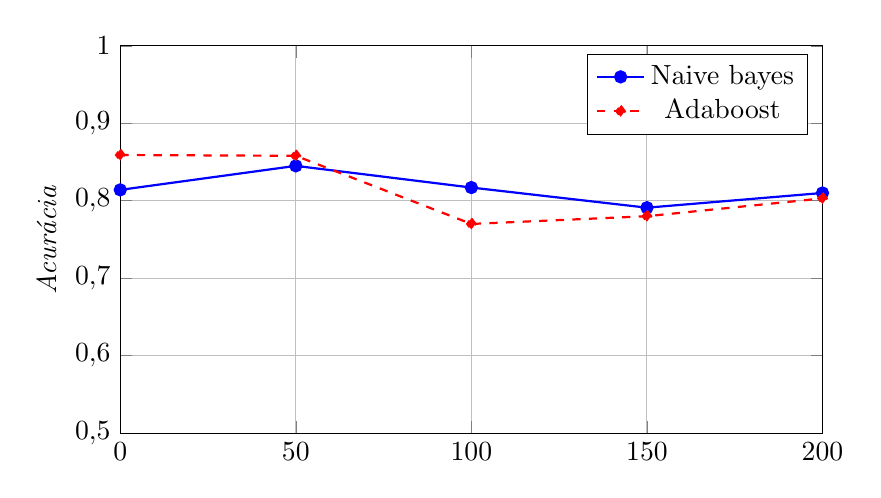
\begin{tikzpicture}
                \begin{axis}[width=10.5cm, 
                        height=6.5cm, 
                        grid=both, 
                        ymin=0.500, ymax=1.000,
                        xmin=0, xmax=200,
                        ylabel={\textit{Acurácia}},
                        % xlabel={Classes},
                        symbolic x coords={0, 50, 100, 150, 200}, 
                        ytick={0.500, 0.600, 0.700, 0.800, 0.900, 1.000},
                        % legend style={at={(0.7,0.9)},anchor=north west},
                        xtick=data
                    ]

                    \addlegendentry{Naive bayes}
                    \addplot[mark=*,thick,blue, solid] coordinates {
                    (0,0.814) 
                    (50,0.845) 
                    (100,0.817) 
                    (150,0.791) 
                    (200,0.810) 
                    };

                    \addlegendentry{Adaboost}
                    \addplot[mark=diamond*,thick,red, dashed] coordinates {
                    (0,0.859) 
                    (50,0.858) 
                    (100,0.770) 
                    (150,0.780) 
                    (200,0.803) 
                    };

                \end{axis}
                \end{tikzpicture}
            \end{center}
            \captionsetup{labelformat=empty}
            \caption{Os pontos da \textit{acurácia} demonstram a \textbf{taxa 
            de acerto}, comprovam que os classificadores \textbf{utilizam 
            corretamente} o \textbf{poder de descriminação} de cada classe da 
            competência III, para a rotulagem de novas amostras.}
            \label{graphic:acuracia}
        \end{figure}
    \end{frame}

    \begin{frame}[fragile]{Matriz de Confusão}
        \begin{table}[H]
            \centering
            \begin{tabular}{cc|c|c|c|c|c|c|}
            \cline{3-8}
             &  & \multicolumn{6}{c|}{\textit{Predição do Naive Bayes}} \\ \cline{3-8} 
             &  & \textbf{0} & \textbf{50} & \textbf{100} & \textbf{150} & \textbf{200} & $\sum_{}$  \\ \hline
            \multicolumn{1}{|c|}{} & \textbf{0} & \cellcolor[HTML]{A8A8A8}63 & 44 & 12 & 12 & 7  & \textit{138} \\ \cline{2-8} 
            \multicolumn{1}{|c|}{} & \textbf{50} & 3  & \cellcolor[HTML]{A8A8A8}99 & 33 & 1  & 2  & \textit{138} \\ \cline{2-8} 
            \multicolumn{1}{|c|}{} & \textbf{100} & 1  & 26 & \cellcolor[HTML]{A8A8A8}82 & 15 & 14 & \textit{138} \\ \cline{2-8} 
            \multicolumn{1}{|c|}{} & \textbf{150} & 3  & 10 & 17 & \cellcolor[HTML]{A8A8A8}61 & 47 & \textit{138} \\ \cline{2-8} 
            \multicolumn{1}{|c|}{} & \textbf{200} & 5  & 13 & 6  & 40 & \cellcolor[HTML]{A8A8A8}74 & \textit{138} \\ \cline{2-8} 
            \multicolumn{1}{|c|}{\multirow{-6}{*}{\textit{\rot{Atual}}}} & $\sum_{}$ & \textit{75} & \textit{192} & \textit{150} & \textit{129} & \textit{144} & \textit{\textbf{690}} \\ \hline
            \end{tabular}
            \captionsetup{labelformat=empty}
            \caption{A matriz de confusão é uma importante ferramenta, na 
            \textbf{avaliação dos resultados} das predições, facilita 
            visualmente o entendimento e \textbf{reage aos efeitos de 
            predições falsas}.}
            \label{tab:matrix_naive_bayes}
        \end{table}
    \end{frame}

    \begin{frame}[fragile]{Matriz de Confusão}
        \begin{table}[H]
            \centering
            \begin{tabular}{cc|c|c|c|c|c|c|}
            \cline{3-8}
             &  & \multicolumn{6}{c|}{\textit{Predição do Naive Bayes}} \\ \cline{3-8} 
             &  & \textbf{0} & \cellcolor[HTML]{f8ff00}\textbf{50} & \textbf{100} & \textbf{150} & \cellcolor[HTML]{f8ff00}\textbf{200} & $\sum_{}$  \\ \hline
            \multicolumn{1}{|c|}{} & \cellcolor[HTML]{f8ff00}\textbf{0} & \cellcolor[HTML]{A8A8A8}63 & \cellcolor[HTML]{f8ff00}44 & 12 & 12 & \cellcolor[HTML]{f8ff00}7  & \textit{138} \\ \cline{2-8} 
            \multicolumn{1}{|c|}{} & \textbf{50} & 3  & \cellcolor[HTML]{A8A8A8}99 & 33 & 1  & 2  & \textit{138} \\ \cline{2-8} 
            \multicolumn{1}{|c|}{} & \textbf{100} & 1  & 26 & \cellcolor[HTML]{A8A8A8}82 & 15 & 14 & \textit{138} \\ \cline{2-8} 
            \multicolumn{1}{|c|}{} & \textbf{150} & 3  & 10 & 17 & \cellcolor[HTML]{A8A8A8}61 & 47 & \textit{138} \\ \cline{2-8} 
            \multicolumn{1}{|c|}{} & \textbf{200} & 5  & 13 & 6  & 40 & \cellcolor[HTML]{A8A8A8}74 & \textit{138} \\ \cline{2-8} 
            \multicolumn{1}{|c|}{\multirow{-6}{*}{\textit{\rot{Atual}}}} & $\sum_{}$ & \textit{75} & \textit{192} & \textit{150} & \textit{129} & \textit{144} & \textit{\textbf{690}} \\ \hline
            \end{tabular}
            \captionsetup{labelformat=empty}
            \caption{A matriz de confusão é uma importante ferramenta, na 
            \textbf{avaliação dos resultados} das predições, facilita 
            visualmente o entendimento e \textbf{reage aos efeitos de 
            predições falsas}.}
            \label{tab:matrix_naive_bayes}
        \end{table}
    \end{frame}

    % \begin{frame}[fragile]{Matriz de Confusão}
    %     \begin{table}[H]
    %         \centering
    %         \begin{tabular}{cc|c|c|c|c|c|c|}
    %         \cline{3-8}
    %          &  & \multicolumn{6}{c|}{\textit{Predição do Naive Bayes}} \\ \cline{3-8} 
    %          &  & \textbf{0} & \textbf{50} & \cellcolor[HTML]{f8ff00}\textbf{100} & \textbf{150} & \cellcolor[HTML]{f8ff00}\textbf{200} & $\sum_{}$  \\ \hline
    %         \multicolumn{1}{|c|}{} & \textbf{0} & \cellcolor[HTML]{A8A8A8}63 & 44 & 12 & 12 & 7  & \textit{138} \\ \cline{2-8} 
    %         \multicolumn{1}{|c|}{} & \cellcolor[HTML]{f8ff00}\textbf{50} & 3  & \cellcolor[HTML]{A8A8A8}99 & \cellcolor[HTML]{f8ff00}33 & 1  & \cellcolor[HTML]{f8ff00}2  & \textit{138} \\ \cline{2-8} 
    %         \multicolumn{1}{|c|}{} & \textbf{100} & 1  & 26 & \cellcolor[HTML]{A8A8A8}82 & 15 & 14 & \textit{138} \\ \cline{2-8} 
    %         \multicolumn{1}{|c|}{} & \textbf{150} & 3  & 10 & 17 & \cellcolor[HTML]{A8A8A8}61 & 47 & \textit{138} \\ \cline{2-8} 
    %         \multicolumn{1}{|c|}{} & \textbf{200} & 5  & 13 & 6  & 40 & \cellcolor[HTML]{A8A8A8}74 & \textit{138} \\ \cline{2-8} 
    %         \multicolumn{1}{|c|}{\multirow{-6}{*}{\textit{\rot{Atual}}}} & $\sum_{}$ & \textit{75} & \textit{192} & \textit{150} & \textit{129} & \textit{144} & \textit{\textbf{690}} \\ \hline
    %         \end{tabular}
    %         \captionsetup{labelformat=empty}
    %         \caption{A matriz de confusão é uma importante ferramenta, na 
    %         \textbf{avaliação dos resultados} das predições, facilita 
    %         visualmente o entendimento e \textbf{reage aos efeitos de 
    %         predições falsas}.}
    %         \label{tab:matrix_naive_bayes}
    %     \end{table}
    % \end{frame}

    \begin{frame}[fragile]{Matriz de Confusão}
        \begin{table}[H]
            \centering
            \begin{tabular}{cc|c|c|c|c|c|c|}
            \cline{3-8}
             &  & \multicolumn{6}{c|}{\textit{Predição do Adaboost}} \\ \cline{3-8} 
             &  & \textbf{0} & \cellcolor[HTML]{f8ff00}\textbf{50} & \textbf{100} & \textbf{150} & \cellcolor[HTML]{f8ff00}\textbf{200} & $\sum_{}$  \\ \hline
            \multicolumn{1}{|c|}{} & \cellcolor[HTML]{f8ff00}\textbf{0} & \cellcolor[HTML]{A8A8A8}99 & \cellcolor[HTML]{f8ff00}18 & 10 & 9  & \cellcolor[HTML]{f8ff00}2  & \textit{138} \\ \cline{2-8} 
            \multicolumn{1}{|c|}{} & \textbf{50} & 20 & \cellcolor[HTML]{A8A8A8}74 & 37 & 6  & 1  & \textit{138} \\ \cline{2-8} 
            \multicolumn{1}{|c|}{} & \textbf{100} & 8  & 27 & \cellcolor[HTML]{A8A8A8}75 & 20 & 8  & \textit{138} \\ \cline{2-8} 
            \multicolumn{1}{|c|}{} & \textbf{150} & 9  & 1  & 18 & \cellcolor[HTML]{A8A8A8}66 & 44 & \textit{138} \\ \cline{2-8} 
            \multicolumn{1}{|c|}{} & \textbf{200} & 7  & 5  & 13 & 50 & \cellcolor[HTML]{A8A8A8}63 & \textit{138} \\ \cline{2-8} 
            \multicolumn{1}{|c|}{\multirow{-6}{*}{\textit{\rot{Atual}}}} & $\sum_{}$ & \textit{143} & \textit{125} & \textit{153} & \textit{151} & \textit{118} & \textit{690} \\ \hline
            \end{tabular}
            \captionsetup{labelformat=empty}
            \caption{Quanto mais \textbf{próximas} as classes, maior é o número 
            de confusões preditas pelos classificadores e quanto mais 
            \textbf{distantes} as classes, menor o número de 
            \textbf{confusões}, ou seja, ambos os classificadores tendem a 
            confundir mais as classes \textbf{0} e \textbf{50}, do que as 
            classes \textbf{0} e \textbf{200}.}
            \label{tab:matrix_adaboost}
        \end{table}
    \end{frame}

    \begin{frame}[fragile]{Padrões Recuperados}
        \pgfplotsset{/pgf/number format/use comma}
        \begin{figure}[H]
            \begin{center}
                \begin{tikzpicture}
                \begin{axis}[
                    width=11.5cm, 
                    height=6.5cm, 
                    grid=both, 
                    ymin=0, ymax=30.000,
                    xmin=0, xmax=75,
                    ylabel={Frequência},
                    ytick={0.000, 5.000, 10.000, 15.000, 20.000, 25.000, 30.000},
                    % xlabel={Índice dos \textit{tokens}},
                    % legend style={at={(0.7,0.9)},anchor=north west}
                    ]
                
                    \addplot [mark=none, color=red, dashed, legend] table[x=x, y=y, col sep=comma]{./data/0.00-0.csv};
                    \addplot [mark=none, color=red, dashed] table[x=x, y=y, col sep=comma]{./data/0.00-1.csv};
                    \addplot [mark=none, color=red, dashed] table[x=x, y=y, col sep=comma]{./data/0.00-2.csv};
                    \addplot [mark=none, color=red, dashed] table[x=x, y=y, col sep=comma]{./data/0.00-3.csv};
                    \addplot [mark=none, color=red, dashed] table[x=x, y=y, col sep=comma]{./data/0.00-4.csv};
                    \addplot [mark=none, color=red, dashed] table[x=x, y=y, col sep=comma]{./data/0.00-5.csv};
                    \addplot [mark=none, color=red, dashed] table[x=x, y=y, col sep=comma]{./data/0.00-6.csv};
                    \addplot [mark=none, color=red, dashed] table[x=x, y=y, col sep=comma]{./data/0.00-7.csv};
                    \addplot [mark=none, color=red, dashed] table[x=x, y=y, col sep=comma]{./data/0.00-8.csv};
                    \addplot [mark=none, color=red, dashed] table[x=x, y=y, col sep=comma]{./data/0.00-9.csv};
                    \addplot [mark=none, color=red, dashed] table[x=x, y=y, col sep=comma]{./data/0.00-10.csv};

                    \addplot [mark=none, color=blue, solid, legend] table[x=x, y=y, col sep=comma]{./data/2.00-0.csv};
                    \addplot [mark=none, color=blue, solid] table[x=x, y=y, col sep=comma]{./data/2.00-1.csv};
                    \addplot [mark=none, color=blue, solid] table[x=x, y=y, col sep=comma]{./data/2.00-2.csv};
                    \addplot [mark=none, color=blue, solid] table[x=x, y=y, col sep=comma]{./data/2.00-3.csv};
                    \addplot [mark=none, color=blue, solid] table[x=x, y=y, col sep=comma]{./data/2.00-4.csv};
                    \addplot [mark=none, color=blue, solid] table[x=x, y=y, col sep=comma]{./data/2.00-5.csv};
                    \addplot [mark=none, color=blue, solid] table[x=x, y=y, col sep=comma]{./data/2.00-6.csv};
                    \addplot [mark=none, color=blue, solid] table[x=x, y=y, col sep=comma]{./data/2.00-7.csv};
                    \addplot [mark=none, color=blue, solid] table[x=x, y=y, col sep=comma]{./data/2.00-8.csv};
                    \addplot [mark=none, color=blue, solid] table[x=x, y=y, col sep=comma]{./data/2.00-9.csv};
                    \addplot [mark=none, color=blue, solid] table[x=x, y=y, col sep=comma]{./data/2.00-10.csv};
                    \legend{Classe 0,,,,,,,,,,, Classe 200,,,,,,,,,,};
                \end{axis}
                \end{tikzpicture}
            \end{center}
            \captionsetup{labelformat=empty}
            \caption{Ambos os padrões possuem \textbf{comportamentos similares}, 
            entretanto, a \textbf{frequência} das palavras utilizadas 
            \textbf{oscilam} em cada classe, o que demonstra a presença do 
            padrão em cada redação.}
            \label{graphic:padrao}
        \end{figure}
    \end{frame}